\documentclass[journal,twoside,web]{ieeecolor}
\usepackage{generic}
% \usepackage{cite}
\usepackage{amsmath,amssymb,amsfonts}
\usepackage{algorithmic}
\usepackage{graphicx}
\usepackage{textcomp}



\usepackage{booktabs}
\usepackage{xcolor}
\usepackage{colortbl}
\usepackage{rotating}
\usepackage{multirow}

\usepackage{biblatex} %Imports biblatex package
\addbibresource{zotero.bib} %Import the bibliography file


% \def\BibTeX{{\rm B\kern-.05em{\sc i\kern-.025em b}\kern-.08em
%     T\kern-.1667em\lower.7ex\hbox{E}\kern-.125emX}}




\markboth{\journalname, VOL. XX, NO. XX, XXXX 2017}
{Author \MakeLowercase{\textit{et al.}}: Point-process based representation learning for Electronic Health Records}
\begin{document}
\title{Point-process based representation learning for Electronic Health Records}
\author{Hojjat Karami, \IEEEmembership{Fellow, IEEE}, Anisoara Ionescu, and David Atienza, \IEEEmembership{Member, IEEE}
\thanks{This paragraph of the first footnote will contain the date on 
which you submitted your paper for review. It will also contain support 
information, including sponsor and financial support acknowledgment. For 
example, ``This work was supported by DigiPredict Grant BS123456.'' }
\thanks{H. Karami is with the EPFL, Lausanne, Switzerland (e-mail: hojjat.karami@epfl.ch). }
\thanks{S. B. Author, Jr., was with Rice University, Houston, TX 77005 USA. He is 
now with the Department of Physics, Colorado State University, Fort Collins, 
CO 80523 USA (e-mail: author@lamar.colostate.edu).}
\thanks{T. C. Author is with 
the Electrical Engineering Department, University of Colorado, Boulder, CO 
80309 USA, on leave from the National Research Institute for Metals, 
Tsukuba, Japan (e-mail: author@nrim.go.jp).}}

\maketitle


\begin{abstract}

    Irregular  sampling of time series in electronic health records (EHRs) is challenging for model development. In addition, the pattern of missingness for certain clinical variables are not at random as it is determined by clinicians decision and the state of patient. Point process is a mathematical framework for handling event sequence data which is also consistent with the irregular sampling. We propose \emph{TEEDAM}, a deep neural network that can learn patient representation from irregulary sample time series as well as informative missingness pattern of certain laboratory variables. We performed various experiments to show the effectiveness of event and state encoding for characterization of conditional intensity functions as well as downstream prediction task. Results show that in some cases learning from patterns may improve the performance of prediction task.
\end{abstract}

\begin{IEEEkeywords}
    electronic health records (EHRs), Point Process, irregular sampling, informative missingness,
\end{IEEEkeywords}


\section{Introduction}
\label{sec:intro}



healthcare systems are one of main area for deploying machine learning models. Thanks to recent advancements in data collection technologies, policies and computing power data are recorded in a hosptial. This data consists of multiple modalities frome tabular and time series to clinical notes and images. We focus on tabular and time series. \cite{zuoTransformerHawkesProcess2020a}


talk about the irregular sampling in EHRs and causes.///
In and ideal setup, variables are measured on a regular basis, however, in a hospital due to medical costs, patient associated risks, sampling device.

conseq of irr sampling/// Irregularly sampled time series in electronic health records can have serious consequences for data analysis and decision making. Irregular sampling occurs when the time intervals between data points are inconsistent, which can lead to biased or inaccurate results when trying to make inferences about the underlying process. This can also make it difficult to accurately compare the data over time, as well as to detect patterns or trends. Furthermore, irregular sampling can cause problems for machine learning algorithms, which may struggle to accurately capture the relationships between variables in the data. This can result in poor predictions or incorrect diagnoses, potentially leading to negative impacts on patient care. To mitigate these consequences, it is important to ensure that electronic health records are sampled at regular intervals, or that appropriate statistical techniques are applied to account for the irregularity.

potential adv of irr sampl/// 

imputation methods/// Imputation techniques are widely used in electronic health records (EHRs) to handle missing data. EHRs often contain incomplete or missing information due to various reasons such as measurement errors, system failures, or data entry issues. Imputation refers to the process of filling in the missing data with plausible values based on the available information. There are several imputation techniques available, each with their own strengths and weaknesses. For example, mean imputation replaces missing values with the mean of the available values in the same column, while regression imputation uses a regression model to estimate the missing values based on the relationship between the variables. Other popular imputation methods include multiple imputation, hot deck imputation, and k-nearest neighbors imputation. The choice of imputation technique depends on the type and amount of missing data, as well as the goals of the analysis. Regardless of the technique used, it is important to carefully consider the impact of imputed values on the analysis and to report the imputation method used in the results.

inherently compatible methods/// Deep learning models that are compatible with irregularly sampled time series are important in many real-world applications, such as stock market predictions, speech recognition, and medical diagnosis. These models need to be able to handle data that is not evenly spaced, as is often the case in time-sensitive applications. One popular deep learning architecture that can handle irregularly sampled time series is the Recurrent Neural Network (RNN). RNNs are well-suited for this task because they have the ability to process sequential data, taking into account not only the current input but also the previous inputs. Another architecture that can handle irregularly sampled time series is the Convolutional Neural Network (CNN), which can be used to extract features from the data and then pass the processed data to an RNN for further analysis. Additionally, Attention Mechanisms can be integrated into RNNs and CNNs to help the model focus on important features in the data. Overall, these deep learning models offer a powerful toolset for handling irregularly sampled time series and provide useful insights into this type of data.


pp framework/// Point processes are mathematical models used to describe the distribution of events in time or space. These events can be occurrences of earthquakes, nerve impulses, customer purchases, or anything else that can be counted or measured. Neural Point Processes are a type of machine learning models that learn the patterns and relationships between events using artificial neural networks. These models can be used for tasks such as predicting future events, estimating the rate of event occurrence, or identifying correlations between events. They offer a flexible and powerful way to analyze point process data, as they can handle complex dependencies between events and incorporate prior knowledge about the process.

Our aims??// In this work, we propose a DNN for joint modeling of NTPP and a DAM. Our first aim is to investigate the effectiveness of state encoding for CIF characterization. Second, we are interested in seeing the utility of event encoding a downstream task

contribs?/// 







\section{Background}
\label{sec:Background}










\subsubsection*{Temporal point process}


Consider an event sequence data  $\mathcal{D}=\{\mathcal{S}_{i}\}_{i=1}^N$ where each sample is represented as an event sequence  $\mathcal{S}_{i}=\{(t_i,e_i)\}_{j=1}^L$, where $L$ is the total number of events, $t_j$ is event's timestamp, and $e_j \in \mathbb{R}^M $ is the binary represntation of event marks (multi-class or multi-label). The history of events is denoted as $\mathcal{H}_t=\{(t_j,e_j):t_j<t \}$.

The core idea of the point process framework is the definition of conditional intensity functions (CIFs) which is the probability of the occurence of an event of type $m$ in an infinitesimal time window $[t,t+dt)$:

\begin{equation} 
   \lambda_m^{*}(t)=\lim \frac{P(  \text{event of type m in } [t,t+\Delta t) |   \mathcal{H}_t  )}{\Delta t} 
\end{equation} 

Multivariate Hawkes process is the traditional approach to characterize CIFs:

\begin{equation} 
    \lambda_m^{*}(t)= \mu_m + \sum_{(t^{\prime},e^{\prime})\in \mathcal{H}_t} \phi(t-t^{\prime})
 \end{equation} 


\subsubsection*{Neural temporal point process}

Encoder-decoder architectures have proven to be effective in many applications. The main idea of a neural temporal point process (NTPP) is to first encode the history of events until $t_j$ using a neural network architecture $h_j=Enc(\mathcal{H}_{j+1};\theta)$. Then it tries to estimate $\lambda^*_m(t)=Dec(h_j;\phi)$ for $ t \in (t_j,t_{j+1}]$.

Initial works used recurrent neural networks either in a discrete way [16], a continuous way [39], or a multi-scale multi-channel architecture [24]; then self-attention was also used by [54, 57]. [57] develop a Structured Transformer Hawkes (STH) model that studies the relationship between point processes. It assumes the modeling of one point process might contribute to the modeling of another. Each vertex in the STH’s graph is associated with a point process. Other efforts have been made to model the cumulative intensity function [42] and conditional probability density [46]. One issue that has been ignored in these works is that these NPP models take all types of historic events to predict the future ones, neglecting that some event types may not contribute to the prediction of another type. This study aims to correct this defect by learning to omit those non-contributing event types when predicting the target type via NPPs.

\subsubsection*{Parameter Estimation}

Based on conditional intensity function, it is straightforward to derive conditional probability density function $p^{*}_{m}(t)$ in $(t_j, t_{j+1}]$:

\begin{equation} 
    p_m^{*}(t)=\lambda_m^{*}(t) \exp \left[-\sum_{m=1}^{M} \int_{t_j}^{t_{j+1}}\lambda_m^{*}(t^{\prime})dt^{\prime}\right]
 \end{equation}
 
 Intuitively, the integral term indicates that there is no event of any type in the interval.

In the multi-class setting, the log-likelihood (LL) of a point process for a single event sequnce $\mathcal{S}_{i}$ is defined as:

\begin{multline} 
    \log p_{mc}(\mathcal{S}_{i})  =  \sum_{j = 1}^{L}\sum_{m = 1}^{M} 1(e_j=m)   \log p_m^{*}(t_j) \\   
    = \sum_{j = 1}^{L}\sum_{m = 1}^{M} 1(e_j=m)   \log \lambda_m^{*}(t_j)\\
    \sum_{m = 1}^{M} \left(   \int_{0}^{T}  \lambda_m^{*}(s) \,ds  \right)
\end{multline} 

However, in many cases such as EHRs it is common to have co-occuring events. [ntpp] proposed to add:

% If we assume that marks and events are independent, 

% \begin{multline} 
%     -\log p(\mathcal{S}_{i})  = \\
%       - \sum_{j = 1}^{L}\sum_{m = 1}^{M} 1(e_j=m)   \log p^{*}(e_j=m) \lambda^{*}(t_j) \\   
%     + \sum_{m = 1}^{M} p^{*}(e_j=m) \left(   \int_{0}^{T}  \lambda_m^{*}(s) \,ds  \right)
% \end{multline} 



\begin{multline} 
    \log p_{ml}(\mathcal{S}_{i}) = \log p_{mc}(\mathcal{S}_{i}) \\
    + \sum_{m = 1}^{M} (1-1(e_j=m)) \log \left(1-p_m^{*}(t_j)  \right)
\end{multline} 


% \begin{multline} 
%     -\log p(\mathcal{S}_{i})  =  - \sum_{j = 1}^{L}\sum_{m = 1}^{M} 1(e_j=m)   \log \lambda_m^{*}(t_j) \\   
%     + \sum_{m = 1}^{M} \left(   \int_{0}^{T}  \lambda_m^{*}(s) \,ds  \right)\\
%     - \sum_{j = 1}^{L}\sum_{m = 1}^{M} (1-1(e_j=m)) \log \left(1-\lambda_m^{*}(t_j) \exp \left( - \int_{0}^{T}  \lambda_m^{*}(s) \,ds  \right) \right)
% \end{multline} 

It should be noted that the real advantage of point process is modeling non-event likelihoods in the form of integrals. If we neglect the integrals, we would achieve the cross-entropy and binary cross entropy loss in the multi-class and multi-label settings respectively for the prediction of next mark given history of events.

Another approach is the marked case which assumes that marks and timestamps are conditionally independent given $\mathcal{H}_t$.

\begin{multline} 
    \log p_{marked}(\mathcal{S}_{i}) =    
    \sum_{j = 1}^{L}\sum_{m = 1}^{M} 1(e_j=m)   \log p^{*}(e_j=m) \\
    +\sum_{j = 1}^{L}\lambda^{*}(t_j) - \int_{t_0}^{t_{L}}\lambda^{*}(t^{\prime})dt^{\prime}  
\end{multline} 

\subsubsection*{Deep learning for irregular sampling}
An irregularly sampled data can be denoted as $\mathcal{D}=\{\mathcal{U}_i\}_{i=1}^{N}$ where $N$ is number of samples and each sample is represented as series of tuple $\mathcal{U}_i={(t_p,k_p,v_p)}$ where $t_p, k_p, v_p$ represents the time, modality and value of $p$-th datapoint respectively.

\section{Related Works}
\label{sec:Related Works}

\section{Proposed Model}
\label{sec:Proposed Model}


\begin{figure*}[!t]
\centerline{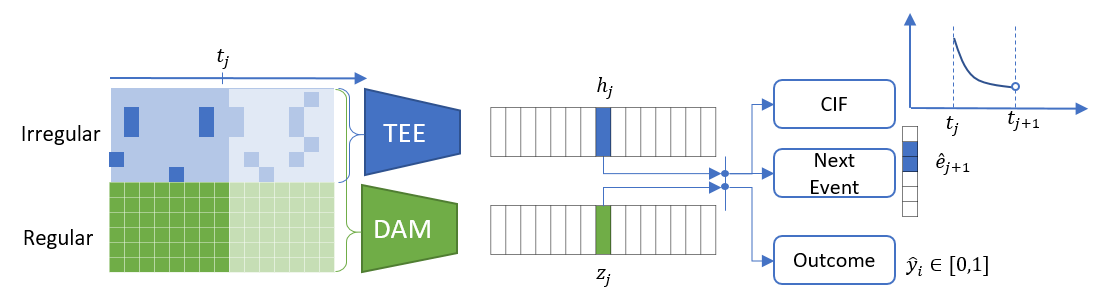
\includegraphics{images/model_arch.png}}
\caption{Magnetization as a function of applied field.
It is good practice to explain the significance of the figure in the caption.}
\label{fig1}
\end{figure*}

 The key advantage of our proposed model is to combine a  transformer-based event encoder (TEE) with a deep attention module (DAM) that can handle an irregularly sampled time series for a any downstream prediciton task. In this case the data is represented as $\mathcal{D}=\{\mathcal{S}_i,\mathcal{U}_i\}_{i=1}^{N}$. General schematic of TEDAM is depicted in FIG.





\subsection{Event Encoder}
We use a similar transformer architecture [thp] for encoding events with minor modifications for event embedding.


In the first step, we embed all event marks $E_{emb}=E \times W_{emb}$ where $E_i \in \mathbb{R}^{L \times M}$ is the binary encoding matrix of all event marks (multi-label or multi-class), and  $ W_{emb} \in  \mathbb{R}^{M \times d_{emb} }  $ is the trainable embedding matrix. 

In the second step, timestamps should be encoded and added to the event embedding, however, we propose to concatenate time encodings that can lead to better characterization of conditional intensity functions. Finally, the input of the transformer encoder will be $X_{emb}=[E_{emb}, T_{emb}] \in \mathbb{R}^{L \times (d_{emb}+t_{emb})}$.

Here, we use the standard transformer encoder similar to [vaswani] with masking matrix to prevent the model from looking into the future. we obtain the encoded matrix  $ H=(h_1, ..., h_j, ..., h_L) $ where $h_j$ containes the all available information until occurence of $j$-th event.






\subsection{State Encoder}

Similar to [setF], we use an attention-based aggregation approach for encoding all additional information. Each side information  $ (t_k, v_k, m_k) $ can be represented by $s_k=(z(t_k), v_k, m_k)$. we define attention $a(\mathcal{U}_k,s_k )$

We define $\mathcal{U}_p$ to be the set of the first $p$ available information.
The goal is to calculate $a(\mathcal{U}_p,s_k ), k \leq p$ that is the relevance of $k$-th observation $s_k$ to the first $p$ observed values $\mathcal{U}_p$.
This is achieved by computing an embedding of the set elements using a smaller set functions $f^{\prime}$, and projecting the concatenation of the set representation and the individual set element into d-dimensional space:



\begin{equation}
    f^{\prime}(\mathcal{U}_p) = g^{\prime} \left(  \frac{1}{|p|} \sum_{u_k \in \mathcal{U}_p}  h^{\prime}(u_k;\theta^{\prime}) ;\rho^{\prime}\right) 
\end{equation}

Then we can compute key values using key matrix $W^k \in \mathbb{R}^{(d_g+d_s) \times d_{prod}}$


\begin{equation}
    K_p=[f^{\prime}(\mathcal{U}_p), u_p]^T W^K   
\end{equation}

using a query vector $w^q \in \mathbb{R}^{d_{prod}}$

\begin{equation*}
    a(\mathcal{U}_p,u_p)=  softmax(\frac{K_p.w^q}{\sqrt{d}  })
\end{equation*}


Finally, we compute a weighted aggregation of set elements:

\begin{equation*}
    z_p = f(\mathcal{U}_p) =     
    g\left(
    \sum_{s_k \in \mathcal{U}_p}  a(\mathcal{U}_p,s_k)h(s_k;\theta);\rho 
    \right) 
\end{equation*}

we regard $z_p \in \mathbb{R}^{d_{\rho}}$ as the representation of state data until arrival of $p$-th datapoint.


Finally, we need to combine event embeddings $ H_{L \times d_e}$ and state embeddings $Z_{P \times d_{\rho}}$, however, the length of each does not match. As a result, we consider the reduced version of state matrix as below:

\begin{equation*}
    Z^{red}_i=Z_p \text{ where } p=argmax(z \leq i)
\end{equation*}





Without loss of generality, we can consider multiple heads by adding an additional dimension to keys and queries.\\


\subsection{All formulas}

% \begin{equation*}
%     \begin{cases} 


% f^{\prime}(\mathcal{S}_p) = g^{\prime} \left(   
%  \frac{1}{p} \sum_{s_k \in \mathcal{S}_p}  h^{\prime}_{\theta}(s_k) 
% \right) \\


% K_p=[f^{\prime}(\mathcal{S}_p), s_p]^T W^K \\
% e_p=\frac{K_p.w^q}{\sqrt{d}  }\\


% a(\mathcal{S}_p,s_k)=\frac{\exp (e_p)}{\sum_{k\leq p} \exp (e_k)  } \\


% f(\mathcal{S}_p) = \sum_{s_k \in \mathcal{S}_p}  a(\mathcal{S}_p,s_k)h_{\theta}(s_k) \\


% z_p=g_{\psi}\left(         f(\mathcal{S}_p)         \right) \\



% \end{cases} 
% \end{equation*}

% \begin{equation}\label{eq:1}
%     [z(t_j)]_{k} = 
%      \begin{cases} 
%         \sin\left(  \frac{t_j}{\mathcal{T}^{(k-1)/d_t} }  \right) & \text{if } k \text{ is odd}\\
%         \sin\left(  \frac{t_j}{\mathcal{T}^{k/d_t} }  \right) & \text{if } k \text{ is even}

%         \end{cases} 
% \end{equation} 
% \begin{equation}
%     \lambda_k(t|\mathcal{H}_t ) = f_k\left(\alpha_k \frac{t-t_j}{t_j}+\mathbf{w}_k^T \mathbf{x}_{enc}(t_j)+\mathbf{y}_k^T \mathbf{s}_{enc}(t_j) +b_k   \right)
% \end{equation}

% \begin{equation}
%     \lambda_k(t|\mathcal{H}_t ) = f_k\left(\alpha_k \frac{t-t_j}{t_j}+\mathbf{w}_k^T \mathbf{x}_{enc}(t_j)+b_k   \right)
% \end{equation}

\subsection{Event Decoder}
Once we obtain a representation of a patient using embedded events and states, we can try to parameterize conditional intensity functions (CIFs) of the events.

In neural point process literature, many approaches have been propose to decode either conditional or cumulative intensity function. We will use a decoder similar to [sahp] as it can model both exciting and inhibiting effects for modeling CIFs.

% \begin{gather*} 
%    \mu_{m,i+1}=gelu(h_{i+1}W_{m,\mu}), 
% \end{gather*}

\begin{gather*} 
    \mu_{m,i+1}=gelu(h_{i+1}W_{m,\mu}  +  z_{i+1}W_{m,\mu}), \\ 
    \eta_{m,i+1}=gelu(h_{i+1}W_{m,\eta}  +  z_{i+1}W_{m,\eta}), \\
    \gamma_{m,i+1}=gelu(h_{i+1}W_{m,\gamma}  +  z_{i+1}W_{m,\gamma}),
    \end{gather*}

Finally, we can express the intensity function as follows:

\begin{multline*}
    \lambda_m(t)=\text{softplus}(\mu_{m,i+1}+\\
    (\eta_{m,i+1}- \mu_{m,i+1}) \exp(-\gamma_{m,i+1}(t-t_i))    ),
\end{multline*}

for $t \in (t_i, t_{i+1}]$,where the $softplus$ is used to constrain thei intensity function to be positive.


\subsection{Loss Function}

We define a multi-objective loss function 
$ \mathcal{L}   =   \mathcal{L}_{CIF}   +   \mathcal{L}_{mark}  +   \mathcal{L}_{state}$.





\section{Experiments}
\label{sec:Experiments}

We perform various experiments to show the effectiveness of each component in out model.
\subsection*{Datasets}


To show the utility of time concatenation and marked loss, we consider three datasets:

\textbf{Synthea(\emph{Syn})}.
We used the Synthea simulator (Walonoski et al., 2018) which generates patient-level EHRs using human expert curated Markov processes. Here, we reused the already processed version of this data by [ntpp].

\textbf{ReTweets (\emph{RT})}.
The Retweets dataset contains sequences of tweets, where each sequence contains an origin tweet (i.e., some user initiates a tweet), and some follow-up tweets. We record the time and the user tag of each tweet. Further, users are grouped into three categories based on the number of their followers: “small”, “medium”, and “large”

\textbf{Stackoverflow (\emph{SO})}.
is a question-answering website. The website rewards users with badges to promote engagement in the community, and the same badge can be rewarded multiple times to the same user. We collect data in a two-year period, and we treat each user’s reward history as a sequence. Each event in the sequence signifies receipt of a particular medal.

Furthermore, we consider two EHRs provided by physionet challenge to investigate the advantage of irregular sample and point process modeling in the same time.

\textbf{Physionet 2012 Mortality Prediction Challenge (\emph{P12})}.
The 2012 Physionet challenge dataset (Goldberger et al., 2000),contains 12, 000 ICU stays each of which lasts at least 48 h. For each stay, a set of general descriptors (such as gender or age) are collected at admission time. Depending on the course of the stay and patient status, up to 37 time series variables were measured (e.g. blood pressure, lactate, and respiration rate). While some modalities might be measured in regular time intervals (e.g. hourly or daily), some are only collected when required; moreover, not all variables are available for each stay.

\textbf{Physionet 2019 Sepsis Early Prediction Challenge (\emph{P19})}.
This dataset contains clinical data of about 40k patients in ICU. Clinical data consist of demographics, vital signs and laboratory values as well as sepsis label in a one-hour time grid. Our objective is to predict the timestamp of next lab sampling events as well as measured variables (event marks) given the patient history.



\subsection*{Scenarios}

To show the utility of time concatenation and marked-shp we report the metrics for SO, RT and SYN and compare it with 3 baselines: SAHP, THP, and GRU-CP.

To show the utility of additional information for CIF modeling, we report NLL/events for P12 and P19 in the following conditions: TE, TE+DAM, TE+noise

Finally, we investigate whether point process characterization can be useful in a downstream task or not. As each dataset consists of different hospitals and the pattern of irregular sampling might differ from hosptial to hospital, we assume different settings: single-center, multi-center and external evaluation.



\subsection*{Baselines}

we compare our model against existing models: THP, SAHP, GRU-CP.     

\subsection*{Metrics}
We report the weighted AUPRC, AUROC of next predicted event as well as root mean sqaure error (RMSE) of next measurement interval.
For evaluating the goodness of fit for the parameterized point process, we report normalized negative likelihood normalized by number of ocurred event (NLL/events). Furthermore, we can also evaluate the learned representation of each patient to predict the sepsis label in a binary classification task.

\subsection*{Training Details}
To be completed.
\section{Results and Discussion}
\label{sec:Results and Discussion}


In this section, we present our results regarding the advantage of state and event encoding.

\subsection{Effect of minor improvements}


[TB1] shows the performance metrics of different datasets. 

In general, time concatenation has lead to better F1-score/AUROC as well as LL/events compared to adding time. This idea can be used for future research in NTPPs for better characterization of CIFs.

Another interesting fact is that in some datasets (A, B) next mark prediction has competetive performance compared to the point process loss. However, in many cases, point process loss significantly improves the performance metrics which indicates that modeling non-event likelihood could be beneficial. In addition, we propose to use next-mark prediction case as a baseline.

Another interesting results is that independent assumption in the marked loss may lead to worse performance compared to MC/ML loss.


% Table generated by Excel2LaTeX from sheet 'time concat'
\begin{table*}[htbp]
  \centering
  \caption{Add caption}
    \begin{tabular}{cccccccccccccc}
    \toprule
          &       & \multicolumn{8}{c}{TEEDAM}                                    &       &       &       &  \\
\cmidrule{3-10}          &       & \multicolumn{2}{c}{AE (next mark)} &       & \multicolumn{2}{c}{PP(single+mark)} &       & \multicolumn{2}{c}{PP (MC/ML)} &       &       &       &  \\
\cmidrule{3-4}\cmidrule{6-7}\cmidrule{9-10}    Dataset & Metric & concat & sum   &       & concat & sum   &       & concat & sum   & Latent & SAHP  & THP   & GRU-CP \\
    \midrule
    \multirow{2}[2]{*}{SO} & LL/\#events & ND    & ND    &       & -0.56 & -0.57 &       &       &       & -1.54 & -1.86 & -1.84 & NR \\
          & F1-score & 27.86 & 28.79 &       & 29.10 & 28.95 &       &       &       & 28.34(0.19) & 24.12 & 23.89 & 26 \\
    \midrule
    \multirow{2}[2]{*}{ReTweet (MC)} & LL/\#events & ND    & ND    &       &       &       &       &       &       & -3.89 & -4.56 & -4.57 & NR \\
          & F1-score &       &       &       &       &       &       &       &       & 58.29 & 53.92 & 53.86 & NR \\
    \midrule
    \multirow{2}[2]{*}{Synthea} & LL/\#events & ND    & ND    &       &       &       &       &       &       & ND    & ND    & ND    & NR \\
          & AUROC &       &       &       &       &       &       &       &       & ND    & ND    & ND    & 0.85(.014) \\
    \midrule
    \multirow{2}[2]{*}{ReTweet (ML)} & LL/\#events & ND    & ND    &       & 1.86  & 1.4   &       &       &       & ND    & ND    & ND    & NR \\
          & AUROC & 63.3  & 61.01 &       & 68.7  & 66.2  &       & 73.87 &       & ND    & ND    & ND    & 0.611(0.001) \\
    \bottomrule
    \end{tabular}%
  \label{tab:addlabel}%
\end{table*}%

  
  
  





\subsection{Negative Likelihood with state encoding}

[TB2] shows the result for estimation of negative likelihood for the two datasets. 

In general we can see that using state information results in lower NLL, however, it cannot neccessarily increase the AUROC for next time prediction.

Another observation is that more data will lead to higher LL.




% Table generated by Excel2LaTeX from sheet 'state enc'
\begin{table}[htbp]
    \centering
    \caption{Add caption}
      \begin{tabular}{ccccc}
      \toprule
            &       & \multicolumn{3}{c}{Model} \\
  \cmidrule{3-5}    Dataset & setting & TE    & TE+DAM & TE+noise \\
      \midrule
      \multirow{3}[2]{*}{P12} & sc    & -1.99 & -1.77 & -1.92 \\
            & mc1   & -0.99 & -1.14 & -0.89 \\
            & mc2   & -1.5  & -1.33 & -1.47 \\
      \midrule
      \multirow{3}[2]{*}{P19} & sc    & 0.55 (0.02) & 0.55 (0.02) & 0.55 (0.02) \\
            & mc1   & -1.81 & -1.62 & -1.69 \\
            & mc2   & -2.77 & -2.38 & -2.67 \\
      \bottomrule
      \end{tabular}%
    \label{tab:addlabel}%
  \end{table}%
  




can u provide one example patient?

\subsection{Downstream task}

[TB3] indicates the result for Mortality/sepsis prediction in different settings and hospital centers.

In some cases, incorporating event embeddings can lead to better performance.









% Table generated by Excel2LaTeX from sheet 'Sheet3'
\begin{table*}[htbp]
    \centering
    \caption{Add caption}
      \begin{tabular}{ccccccccccc}
      \toprule
            &       &       & \multicolumn{2}{c}{F1} &       & \multicolumn{2}{c}{AUPRC} &       & \multicolumn{2}{c}{AUROC} \\
  \cmidrule{4-5}\cmidrule{7-8}\cmidrule{10-11}    Dataset & Setting & Center & DAM   & TE+DAM &       & DAM   & TE+DAM &       & DAM   & TE+DAM \\
      \midrule
      \multirow{8}[6]{*}{P12} & \multirow{3}[2]{*}{sc} & 1     & 0.55 (0.02) & 0.55 (0.02) &       & 0.55 (0.02) & 0.55 (0.02) &       & 0.55 (0.02) & 0.55 (0.02) \\
            &       & 2     & 0.55 (0.02) & 0.55 (0.02) &       & 0.55 (0.02) & 0.55 (0.02) &       & 0.55 (0.02) & 0.55 (0.02) \\
            &       & 3     & 0.55 (0.02) & 0.55 (0.02) &       & 0.55 (0.02) & 0.55 (0.02) &       & 0.55 (0.02) & 0.55 (0.02) \\
  \cmidrule{2-11}          & \multirow{3}[2]{*}{mc1} & 1     & 0.55 (0.02) & 0.55 (0.02) &       & 0.55 (0.02) & 0.55 (0.02) &       & 0.55 (0.02) & 0.55 (0.02) \\
            &       & 2     & 0.55 (0.02) & 0.55 (0.02) &       & 0.55 (0.02) & 0.55 (0.02) &       & 0.55 (0.02) & 0.55 (0.02) \\
            &       & 3     & 0.55 (0.02) & 0.55 (0.02) &       & 0.55 (0.02) & 0.55 (0.02) &       & 0.55 (0.02) & 0.55 (0.02) \\
  \cmidrule{2-11}          & mc2   & -     & 0.55 (0.02) & 0.55 (0.02) &       & 0.55 (0.02) & 0.55 (0.02) &       & 0.55 (0.02) & 0.55 (0.02) \\
            & seft  & -     & 0.55 (0.02) & 0.55 (0.02) &       & 0.55 (0.02) & 0.55 (0.02) &       & 0.55 (0.02) & 0.55 (0.02) \\
      \midrule
      \multirow{8}[6]{*}{P19} & \multirow{3}[2]{*}{sc} & 1     & 0.55 (0.02) & 0.55 (0.02) &       & 0.55 (0.02) & 0.55 (0.02) &       & 0.55 (0.02) & 0.55 (0.02) \\
            &       & 2     & 0.55 (0.02) & 0.55 (0.02) &       & 0.55 (0.02) & 0.55 (0.02) &       & 0.55 (0.02) & 0.55 (0.02) \\
            &       & 3     & 0.55 (0.02) & 0.55 (0.02) &       & 0.55 (0.02) & 0.55 (0.02) &       & 0.55 (0.02) & 0.55 (0.02) \\
  \cmidrule{2-11}          & \multirow{3}[2]{*}{mc1} & 1     & 0.55 (0.02) & 0.55 (0.02) &       & 0.55 (0.02) & 0.55 (0.02) &       & 0.55 (0.02) & 0.55 (0.02) \\
            &       & 2     & 0.55 (0.02) & 0.55 (0.02) &       & 0.55 (0.02) & 0.55 (0.02) &       & 0.55 (0.02) & 0.55 (0.02) \\
            &       & 3     & 0.55 (0.02) & 0.55 (0.02) &       & 0.55 (0.02) & 0.55 (0.02) &       & 0.55 (0.02) & 0.55 (0.02) \\
  \cmidrule{2-11}          & mc2   & -     & 0.55 (0.02) & 0.55 (0.02) &       & 0.55 (0.02) & 0.55 (0.02) &       & 0.55 (0.02) & 0.55 (0.02) \\
            & seft  & -     & 0.55 (0.02) & 0.55 (0.02) &       & 0.55 (0.02) & 0.55 (0.02) &       & 0.55 (0.02) & 0.55 (0.02) \\
      \bottomrule
      \end{tabular}%
    \label{tab:addlabel}%
  \end{table*}%
  
  
  
  








\subsection{Learned representions}
Fig 1 visualizes the tsne plot for the two scenarios.


\subsection{Model interpretability}

one advantage of proposed method is use of attention mechanisms in both event and state encoder.
Fig 1 shows the attention mechanism



\subsection{Likelihood estimation}

Although CIF does not improve mark prediction, it has led to better representation of patient for downstream task such as sepsis prediction.

In addition, we can interpret some of learned CIF patterns.

explain the effect of time concatenation in SO dataset



tsne of learned representation. 4 modes:


\begin{itemize}
    \item (DA,TE)->(Mark, CIF)
\end{itemize}

attention of DA for sepsis prediction

attention matrix of events for SO dataset

\section{Conclusion}
\label{sec:Conclusion}








% \begin{thebibliography}{00}

% \bibitem{b1} G. O. Young, ``Synthetic structure of industrial plastics,'' in \emph{Plastics,} 2\textsuperscript{nd} ed., vol. 3, J. Peters, Ed. New York, NY, USA: McGraw-Hill, 1964, pp. 15--64.

% \bibitem{b2} W.-K. Chen, \emph{Linear Networks and Systems.} Belmont, CA, USA: Wadsworth, 1993, pp. 123--135.

% \bibitem{b3} J. U. Duncombe, ``Infrared navigation---Part I: An assessment of feasibility,'' \emph{IEEE Trans. Electron Devices}, vol. ED-11, no. 1, pp. 34--39, Jan. 1959, 10.1109/TED.2016.2628402.

% \bibitem{b4} E. P. Wigner, ``Theory of traveling-wave optical laser,'' \emph{Phys. Rev}., vol. 134, pp. A635--A646, Dec. 1965.

% \bibitem{b5} E. H. Miller, ``A note on reflector arrays,'' \emph{IEEE Trans. Antennas Propagat}., to be published.

% \bibitem{b6} E. E. Reber, R. L. Michell, and C. J. Carter, ``Oxygen absorption in the earth's atmosphere,'' Aerospace Corp., Los Angeles, CA, USA, Tech. Rep. TR-0200 (4230-46)-3, Nov. 1988.

% \bibitem{b7} J. H. Davis and J. R. Cogdell, ``Calibration program for the 16-foot antenna,'' Elect. Eng. Res. Lab., Univ. Texas, Austin, TX, USA, Tech. Memo. NGL-006-69-3, Nov. 15, 1987.

% \bibitem{b8} \emph{Transmission Systems for Communications}, 3\textsuperscript{rd} ed., Western Electric Co., Winston-Salem, NC, USA, 1985, pp. 44--60.

% \bibitem{b9} \emph{Motorola Semiconductor Data Manual}, Motorola Semiconductor Products Inc., Phoenix, AZ, USA, 1989.

% \bibitem{b10} G. O. Young, ``Synthetic structure of industrial
% plastics,'' in Plastics, vol. 3, Polymers of Hexadromicon, J. Peters,
% Ed., 2\textsuperscript{nd} ed. New York, NY, USA: McGraw-Hill, 1964, pp. 15-64.
% [Online]. Available:
% \underline{http://www.bookref.com}.

% \bibitem{b11} \emph{The Founders' Constitution}, Philip B. Kurland
% and Ralph Lerner, eds., Chicago, IL, USA: Univ. Chicago Press, 1987.
% [Online]. Available: \underline{http://press-pubs.uchicago.edu/founders/}

% \bibitem{b12} The Terahertz Wave eBook. ZOmega Terahertz Corp., 2014.
% [Online]. Available:
% \underline{http://dl.z-thz.com/eBook/zomega\_ebook\_pdf\_1206\_sr.pdf}. Accessed on: May 19, 2014.

% \bibitem{b13} Philip B. Kurland and Ralph Lerner, eds., \emph{The
% Founders' Constitution.} Chicago, IL, USA: Univ. of Chicago Press,
% 1987, Accessed on: Feb. 28, 2010, [Online] Available:
% \underline{http://press-pubs.uchicago.edu/founders/}

% \bibitem{b14} J. S. Turner, ``New directions in communications,'' \emph{IEEE J. Sel. Areas Commun}., vol. 13, no. 1, pp. 11-23, Jan. 1995.

% \bibitem{b15} W. P. Risk, G. S. Kino, and H. J. Shaw, ``Fiber-optic frequency shifter using a surface acoustic wave incident at an oblique angle,'' \emph{Opt. Lett.}, vol. 11, no. 2, pp. 115--117, Feb. 1986.

% \bibitem{b16} P. Kopyt \emph{et al., ``}Electric properties of graphene-based conductive layers from DC up to terahertz range,'' \emph{IEEE THz Sci. Technol.,} to be published. DOI: 10.1109/TTHZ.2016.2544142.

% \bibitem{b17} PROCESS Corporation, Boston, MA, USA. Intranets:
% Internet technologies deployed behind the firewall for corporate
% productivity. Presented at INET96 Annual Meeting. [Online].
% Available: \underline{http://home.process.com/Intranets/wp2.htp}

% \bibitem{b18} R. J. Hijmans and J. van Etten, ``Raster: Geographic analysis and modeling with raster data,'' R Package Version 2.0-12, Jan. 12, 2012. [Online]. Available: \underline {http://CRAN.R-project.org/package=raster} 

% \bibitem{b19} Teralyzer. Lytera UG, Kirchhain, Germany [Online].
% Available:
% \underline{http://www.lytera.de/Terahertz\_THz\_Spectroscopy.php?id=home}, Accessed on: Jun. 5, 2014

% \bibitem{b20} U.S. House. 102\textsuperscript{nd} Congress, 1\textsuperscript{st} Session. (1991, Jan. 11). \emph{H. Con. Res. 1, Sense of the Congress on Approval of}  \emph{Military Action}. [Online]. Available: LEXIS Library: GENFED File: BILLS

% \bibitem{b21} Musical toothbrush with mirror, by L.M.R. Brooks. (1992, May 19). Patent D 326 189 [Online]. Available: NEXIS Library: LEXPAT File: DES

% \bibitem{b22} D. B. Payne and J. R. Stern, ``Wavelength-switched pas- sively coupled single-mode optical network,'' in \emph{Proc. IOOC-ECOC,} Boston, MA, USA, 1985, pp. 585--590.

% \bibitem{b23} D. Ebehard and E. Voges, ``Digital single sideband detection for interferometric sensors,'' presented at the \emph{2\textsuperscript{nd} Int. Conf. Optical Fiber Sensors,} Stuttgart, Germany, Jan. 2-5, 1984.

% \bibitem{b24} G. Brandli and M. Dick, ``Alternating current fed power supply,'' U.S. Patent 4 084 217, Nov. 4, 1978.

% \bibitem{b25} J. O. Williams, ``Narrow-band analyzer,'' Ph.D. dissertation, Dept. Elect. Eng., Harvard Univ., Cambridge, MA, USA, 1993.

% \bibitem{b26} N. Kawasaki, ``Parametric study of thermal and chemical nonequilibrium nozzle flow,'' M.S. thesis, Dept. Electron. Eng., Osaka Univ., Osaka, Japan, 1993.

% \bibitem{b27} A. Harrison, private communication, May 1995.

% \bibitem{b28} B. Smith, ``An approach to graphs of linear forms,'' unpublished.

% \bibitem{b29} A. Brahms, ``Representation error for real numbers in binary computer arithmetic,'' IEEE Computer Group Repository, Paper R-67-85.

% \bibitem{b30} IEEE Criteria for Class IE Electric Systems, IEEE Standard 308, 1969.

% \bibitem{b31} Letter Symbols for Quantities, ANSI Standard Y10.5-1968.

% \bibitem{b32} R. Fardel, M. Nagel, F. Nuesch, T. Lippert, and A. Wokaun, ``Fabrication of organic light emitting diode pixels by laser-assisted forward transfer,'' \emph{Appl. Phys. Lett.}, vol. 91, no. 6, Aug. 2007, Art. no. 061103.~

% \bibitem{b33} J. Zhang and N. Tansu, ``Optical gain and laser characteristics of InGaN quantum wells on ternary InGaN substrates,'' \emph{IEEE Photon. J.}, vol. 5, no. 2, Apr. 2013, Art. no. 2600111

% \bibitem{b34} S. Azodolmolky~\emph{et al.}, Experimental demonstration of an impairment aware network planning and operation tool for transparent/translucent optical networks,''~\emph{J. Lightw. Technol.}, vol. 29, no. 4, pp. 439--448, Sep. 2011.

% \end{thebibliography}

\printbibliography




% \begin{IEEEbiography}[{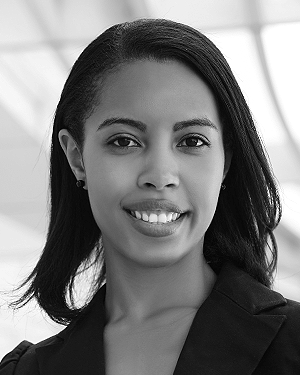
\includegraphics[width=1in,height=1.25in,clip,keepaspectratio]{a1.png}}]{First A. Author} (M'76--SM'81--F'87) and all authors may include 
% biographies. Biographies are often not included in conference-related
% papers. This author became a Member (M) of IEEE in 1976, a Senior
% Member (SM) in 1981, and a Fellow (F) in 1987. The first paragraph may
% contain a place and/or date of birth (list place, then date). Next,
% the author's educational background is listed. The degrees should be
% listed with type of degree in what field, which institution, city,
% state, and country, and year the degree was earned. The author's major
% field of study should be lower-cased. 

% The second paragraph uses the pronoun of the person (he or she) and not the 
% author's last name. It lists military and work experience, including summer 
% and fellowship jobs. Job titles are capitalized. The current job must have a 
% location; previous positions may be listed 
% without one. Information concerning previous publications may be included. 
% Try not to list more than three books or published articles. The format for 
% listing publishers of a book within the biography is: title of book 
% (publisher name, year) similar to a reference. Current and previous research 
% interests end the paragraph. The third paragraph begins with the author's 
% title and last name (e.g., Dr.\ Smith, Prof.\ Jones, Mr.\ Kajor, Ms.\ Hunter). 
% List any memberships in professional societies other than the IEEE. Finally, 
% list any awards and work for IEEE committees and publications. If a 
% photograph is provided, it should be of good quality, and 
% professional-looking. Following are two examples of an author's biography.
% \end{IEEEbiography}

% \begin{IEEEbiography}[{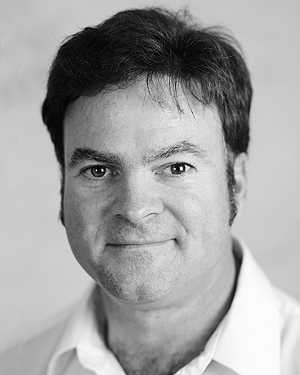
\includegraphics[width=1in,height=1.25in,clip,keepaspectratio]{a2.png}}]{Second B. Author} was born in Greenwich Village, New York, NY, USA in 
% 1977. He received the B.S. and M.S. degrees in aerospace engineering from 
% the University of Virginia, Charlottesville, in 2001 and the Ph.D. degree in 
% mechanical engineering from Drexel University, Philadelphia, PA, in 2008.

% From 2001 to 2004, he was a Research Assistant with the Princeton Plasma 
% Physics Laboratory. Since 2009, he has been an Assistant Professor with the 
% Mechanical Engineering Department, Texas A{\&}M University, College Station. 
% He is the author of three books, more than 150 articles, and more than 70 
% inventions. His research interests include high-pressure and high-density 
% nonthermal plasma discharge processes and applications, microscale plasma 
% discharges, discharges in liquids, spectroscopic diagnostics, plasma 
% propulsion, and innovation plasma applications. He is an Associate Editor of 
% the journal \emph{Earth, Moon, Planets}, and holds two patents. 

% Dr. Author was a recipient of the International Association of Geomagnetism 
% and Aeronomy Young Scientist Award for Excellence in 2008, and the IEEE 
% Electromagnetic Compatibility Society Best Symposium Paper Award in 2011. 
% \end{IEEEbiography}

% \begin{IEEEbiography}[{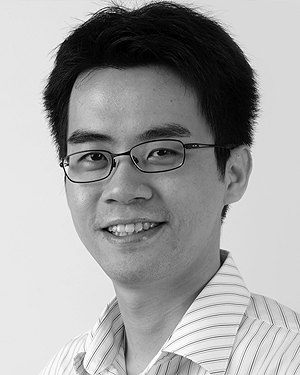
\includegraphics[width=1in,height=1.25in,clip,keepaspectratio]{a3.png}}]{Third C. Author, Jr.} (M'87) received the B.S. degree in mechanical 
% engineering from National Chung Cheng University, Chiayi, Taiwan, in 2004 
% and the M.S. degree in mechanical engineering from National Tsing Hua 
% University, Hsinchu, Taiwan, in 2006. He is currently pursuing the Ph.D. 
% degree in mechanical engineering at Texas A{\&}M University, College 
% Station, TX, USA.

% From 2008 to 2009, he was a Research Assistant with the Institute of 
% Physics, Academia Sinica, Tapei, Taiwan. His research interest includes the 
% development of surface processing and biological/medical treatment 
% techniques using nonthermal atmospheric pressure plasmas, fundamental study 
% of plasma sources, and fabrication of micro- or nanostructured surfaces. 

% Mr. Author's awards and honors include the Frew Fellowship (Australian 
% Academy of Science), the I. I. Rabi Prize (APS), the European Frequency and 
% Time Forum Award, the Carl Zeiss Research Award, the William F. Meggers 
% Award and the Adolph Lomb Medal (OSA).
% \end{IEEEbiography}

\end{document}
